\documentclass{article}
\usepackage{graphicx}
\usepackage{subcaption}

\title{Weekly meeting notes}
\author{Eugenio Pescimoro }

\begin{document}

\maketitle

\section{Introduction}
The aim of these notes is to describe one of the available numerical methods for modelling the diffusion and reaction processes of liquid chemical compounds displacing through fractured porous media.

\section{Diffusion in fractures}
The drifting term..

\section{Code verification}
As a first step for ensuring the reliability of a solute transport simulation code it is essential to verify that the solutions of numerical experiments and analytical study coincide. For this purpose we compare the analytical solutions from three different transport problems against the numerically generated results, namely:
\begin{itemize}
    \item spatial distribution of the concentration at a given time for a solute that is displaced through an infinite bi-dimensional domain with horizontal impenetrable boundaries and initial one-dimensional vertical location;
    \item probability density function of a breakthrough curve for a solute which is displaced through a semi-infinite domain where particles' arriving times are recorded on a vertical absorbing control plane;
    \item degradation curve for a solute travelling through an infinite domain.
\end{itemize}

\subsection{Infinite domain}
\begin{figure}[htbp]
    \centering
    \begin{subfigure}[b]{0.45\textwidth}
        \centering
        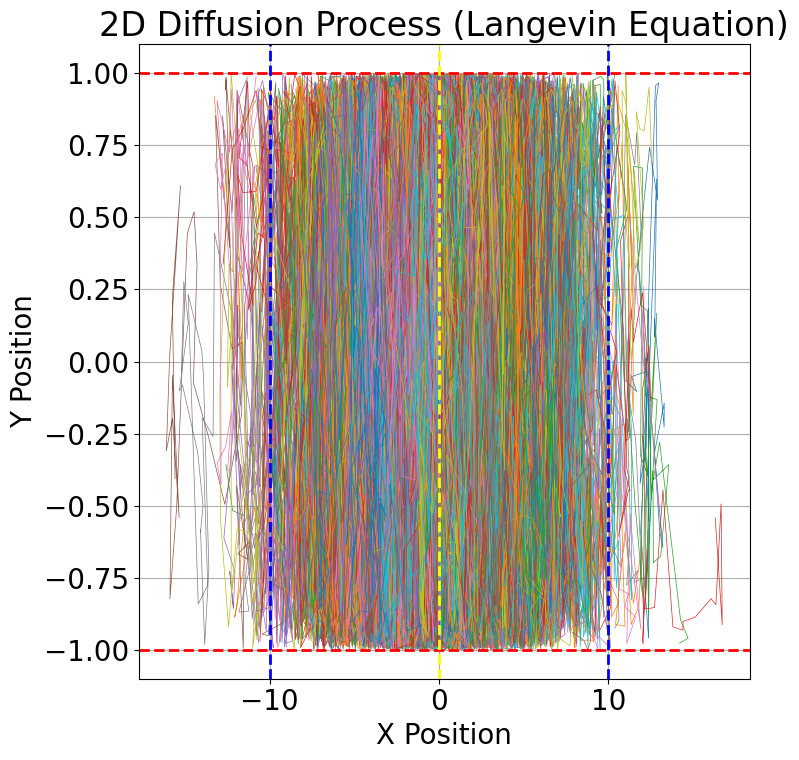
\includegraphics[width=\textwidth]{images/trajectoriesInfinite.png} % Replace with your image path
        \caption{Trajectories of 1e4 particles during 1e3 time steps}
        \label{fig:subplotTrInf}
    \end{subfigure}
    \hfill
    \begin{subfigure}[b]{0.45\textwidth}
        \centering
        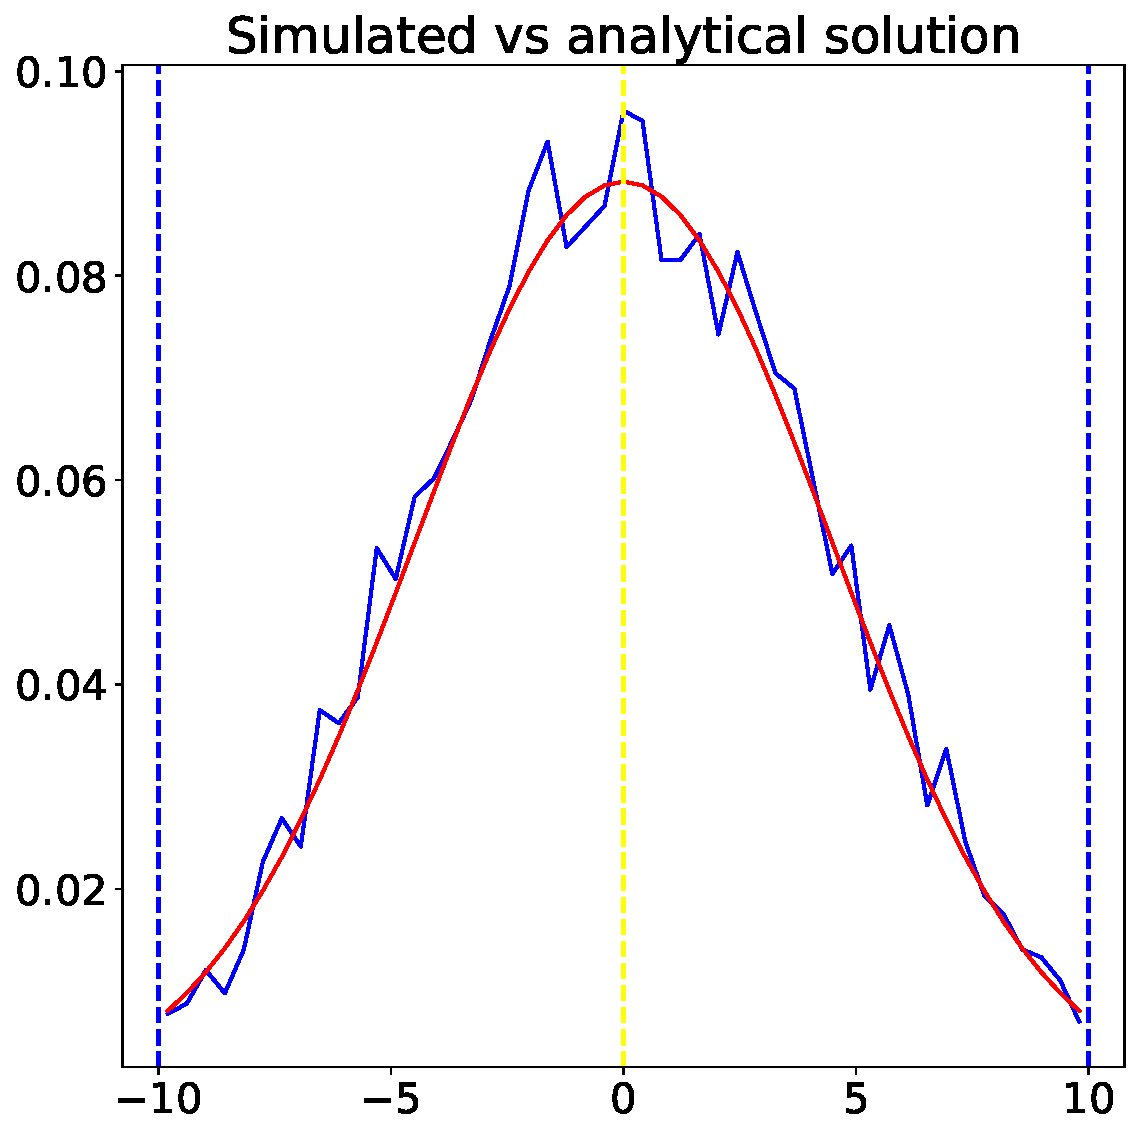
\includegraphics[width=\textwidth]{images/verificationInfinite.pdf} % Replace with your image path
        \caption{Spatial distribution of the particles at time 1e2}
        \label{fig:subplotVerInf}
    \end{subfigure}
    \caption{Verification of the code comparing two spatial distribution of the concentration at a given time: solid blue line represents the spatial concentration from a numerical simulation while solid red line shows the analytical solution of the spatial concentration in a infinite domain at the same given time}
    \label{fig:Infinite}
\end{figure}

\subsection{Semi-infinite domain}
\begin{figure}[htbp]
    \centering
    \begin{subfigure}[b]{0.45\textwidth}
        \centering
        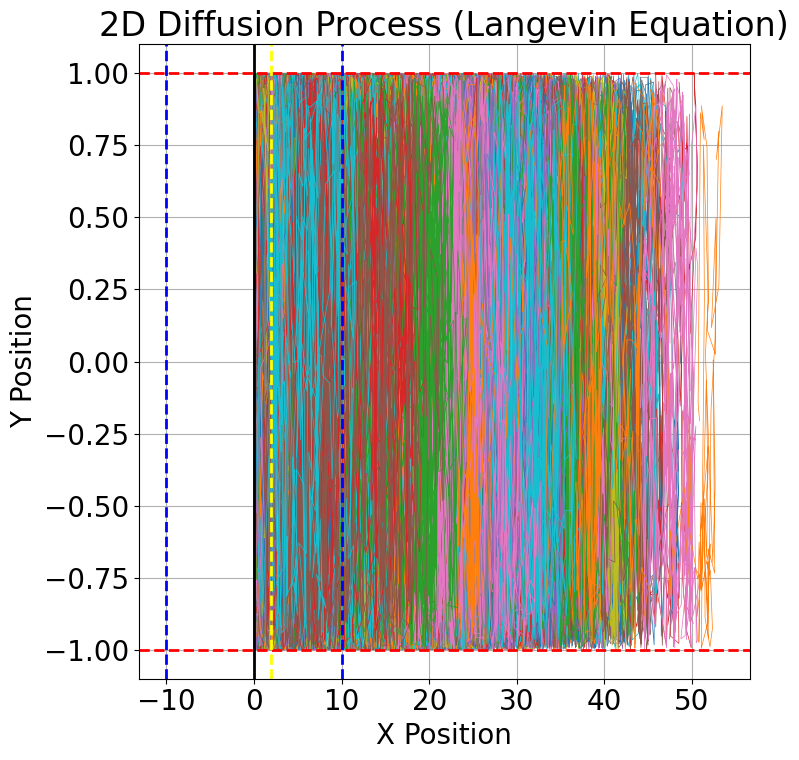
\includegraphics[width=\textwidth]{images/trajectoriesSemiInfinite.png} % Replace with your image path
        \caption{Trajectories of 1e4 particles during 1e3 time steps}
        \label{fig:subplotTrSemiInf}
    \end{subfigure}
    \hfill
    \begin{subfigure}[b]{0.45\textwidth}
        \centering
        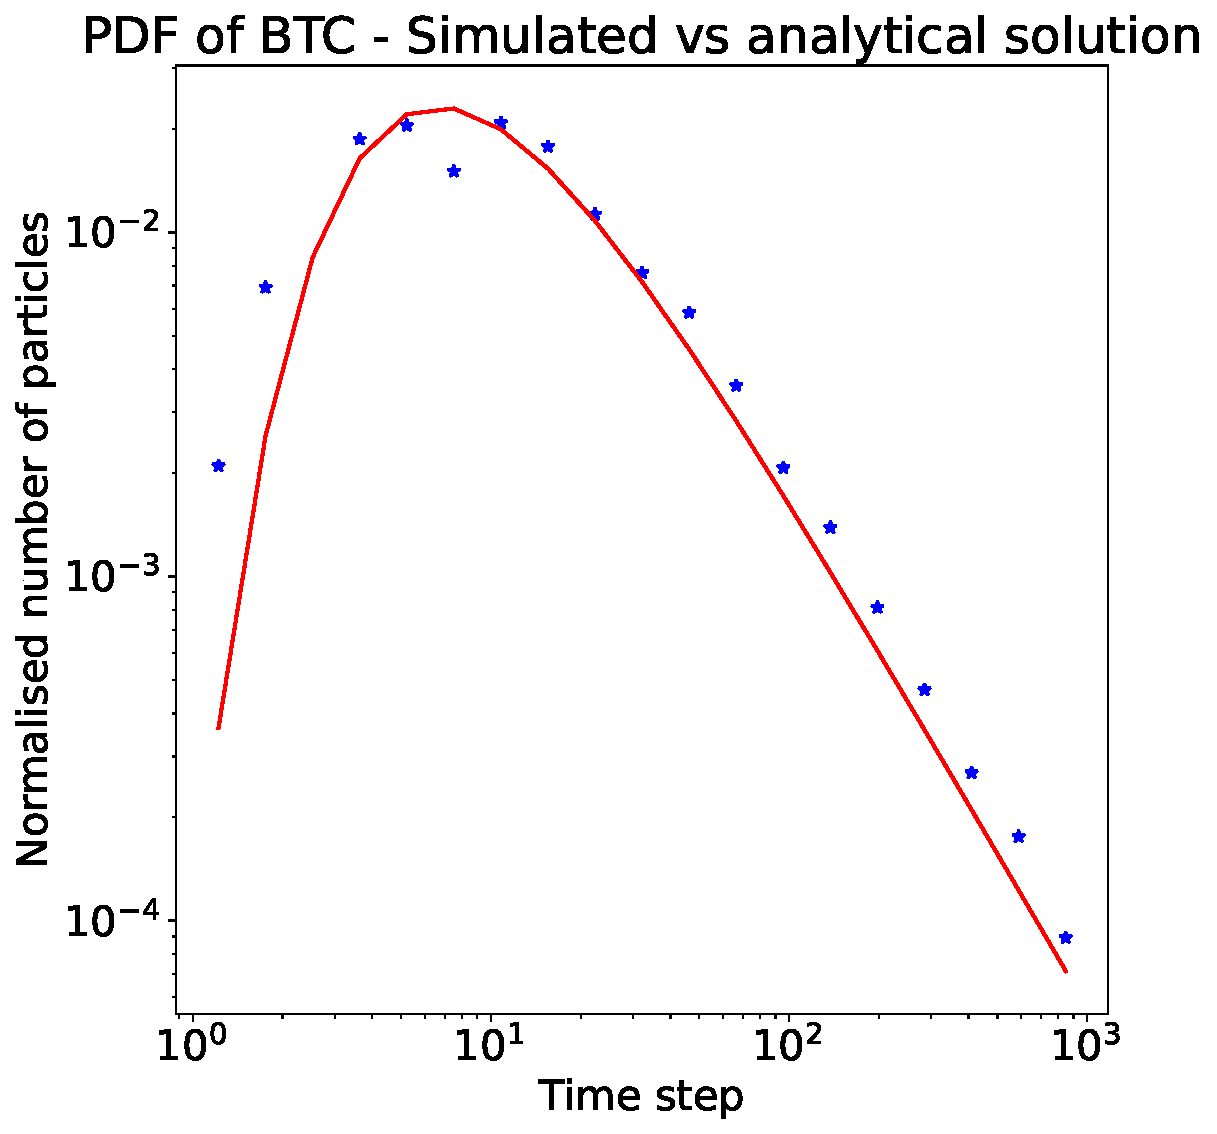
\includegraphics[width=\textwidth]{images/verificationSemi-infinite.pdf} % Replace with your image path
        \caption{Arrival times on the left absorbing boundary}
        \label{fig:subplotVerSemiInf}
    \end{subfigure}
    \caption{Verification of the code comparing two pdfs of the btc: blue dots represent the btc pdf from numerical simulation, solid red line is the analytical solution of the btc pdf for a semi-infinite domain}
    \label{fig:SemiInfinite}
\end{figure}

\subsection{Degradation}
\begin{figure}[htbp]
    \centering
    \begin{subfigure}[b]{0.45\textwidth}
        \centering
        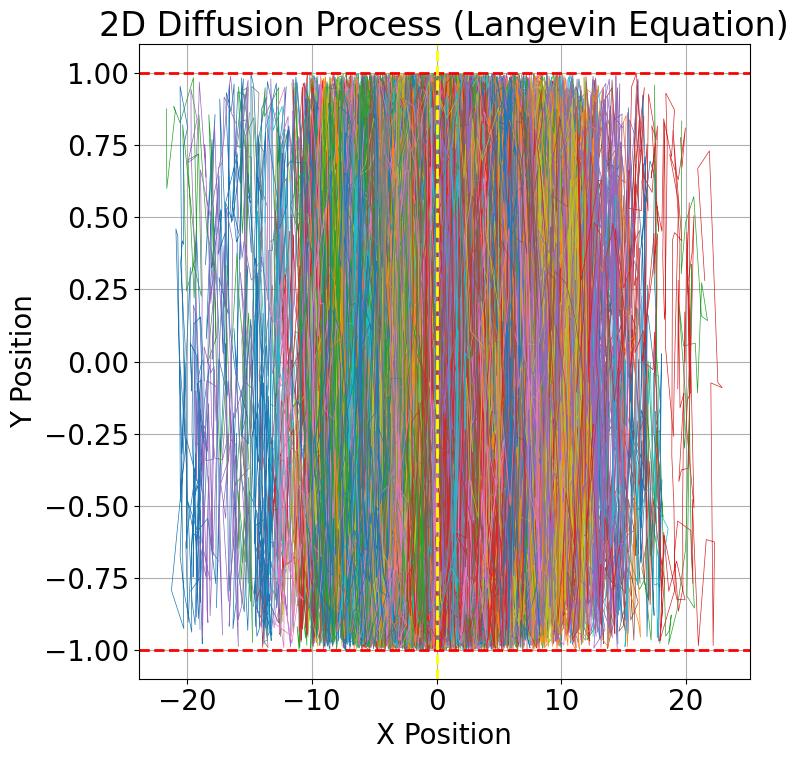
\includegraphics[width=\textwidth]{images/trajectoriesDegradation.png} % Replace with your image path
        \caption{Trajectories of 1e3 particles during 1e3 time steps with degradation}
        \label{fig:subplotTrDeg}
    \end{subfigure}
    \hfill
    \begin{subfigure}[b]{0.45\textwidth}
        \centering
        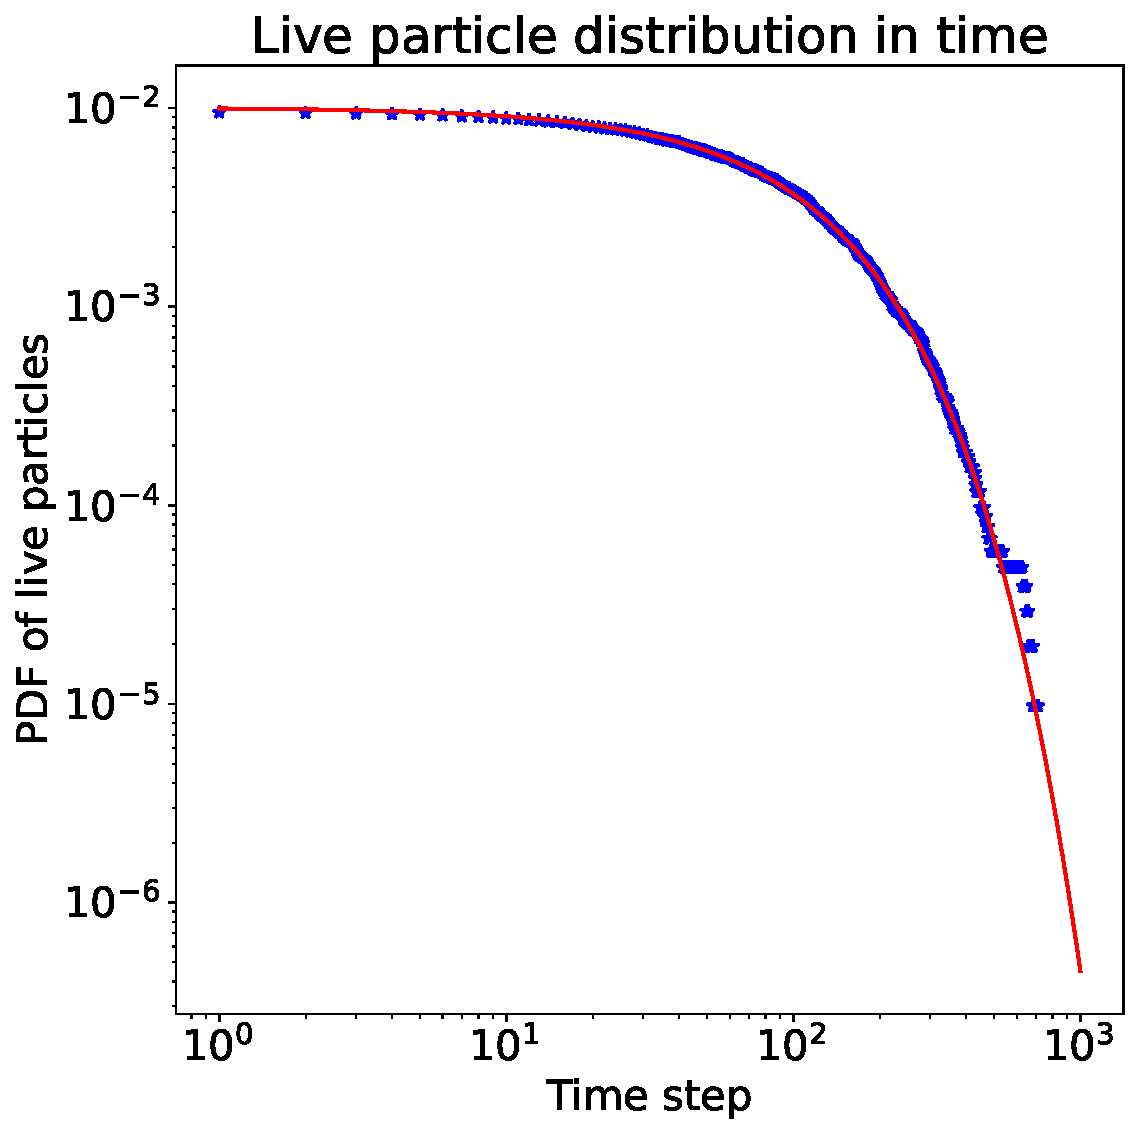
\includegraphics[width=\textwidth]{images/liveParticleInTime.pdf} % Replace with your image path
        \caption{PDF of survived particles in time}
        \label{fig:subplotLivePart}
    \end{subfigure}
    \caption{Verification of the code comparing two pdfs of the btc: blue dots represent the btc pdf from numerical simulation, solid red line is the analytical solution of the btc pdf for a semi-infinite domain}
    \label{fig:Degradation}
\end{figure}

\section{Absorbing boundaries}
\subsection{Final positions}
\begin{figure}[h]
    \centering
    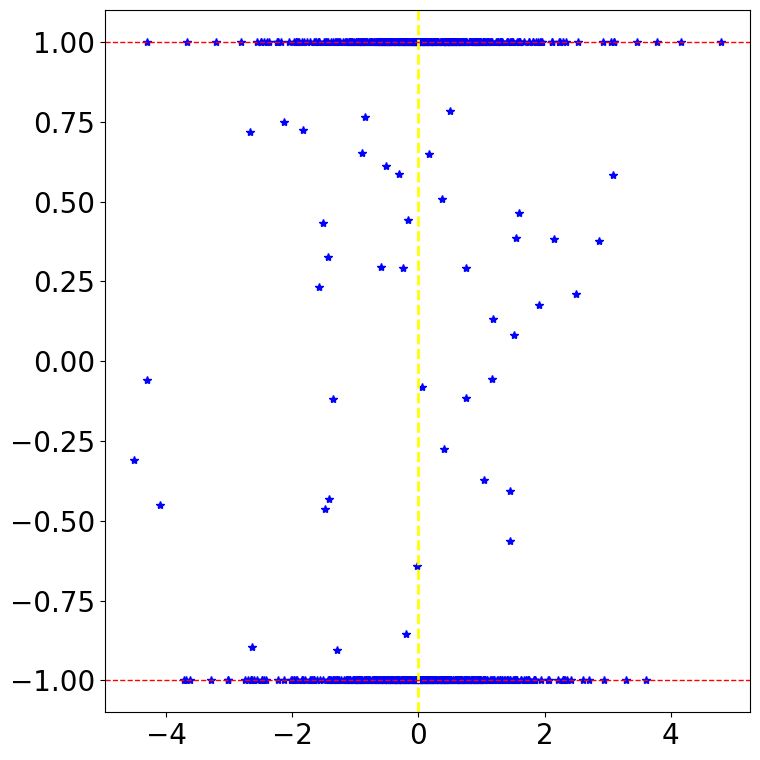
\includegraphics[width=0.5\textwidth]{images/finalPositions.png}
    \caption{Final position for 1e4 particles after 20 steps in a domain characterised by absorbing boundaries}
    \label{fig:finalPos}
\end{figure}

\begin{figure}[htbp]
    \centering
    \begin{subfigure}[b]{0.45\textwidth}
        \centering
        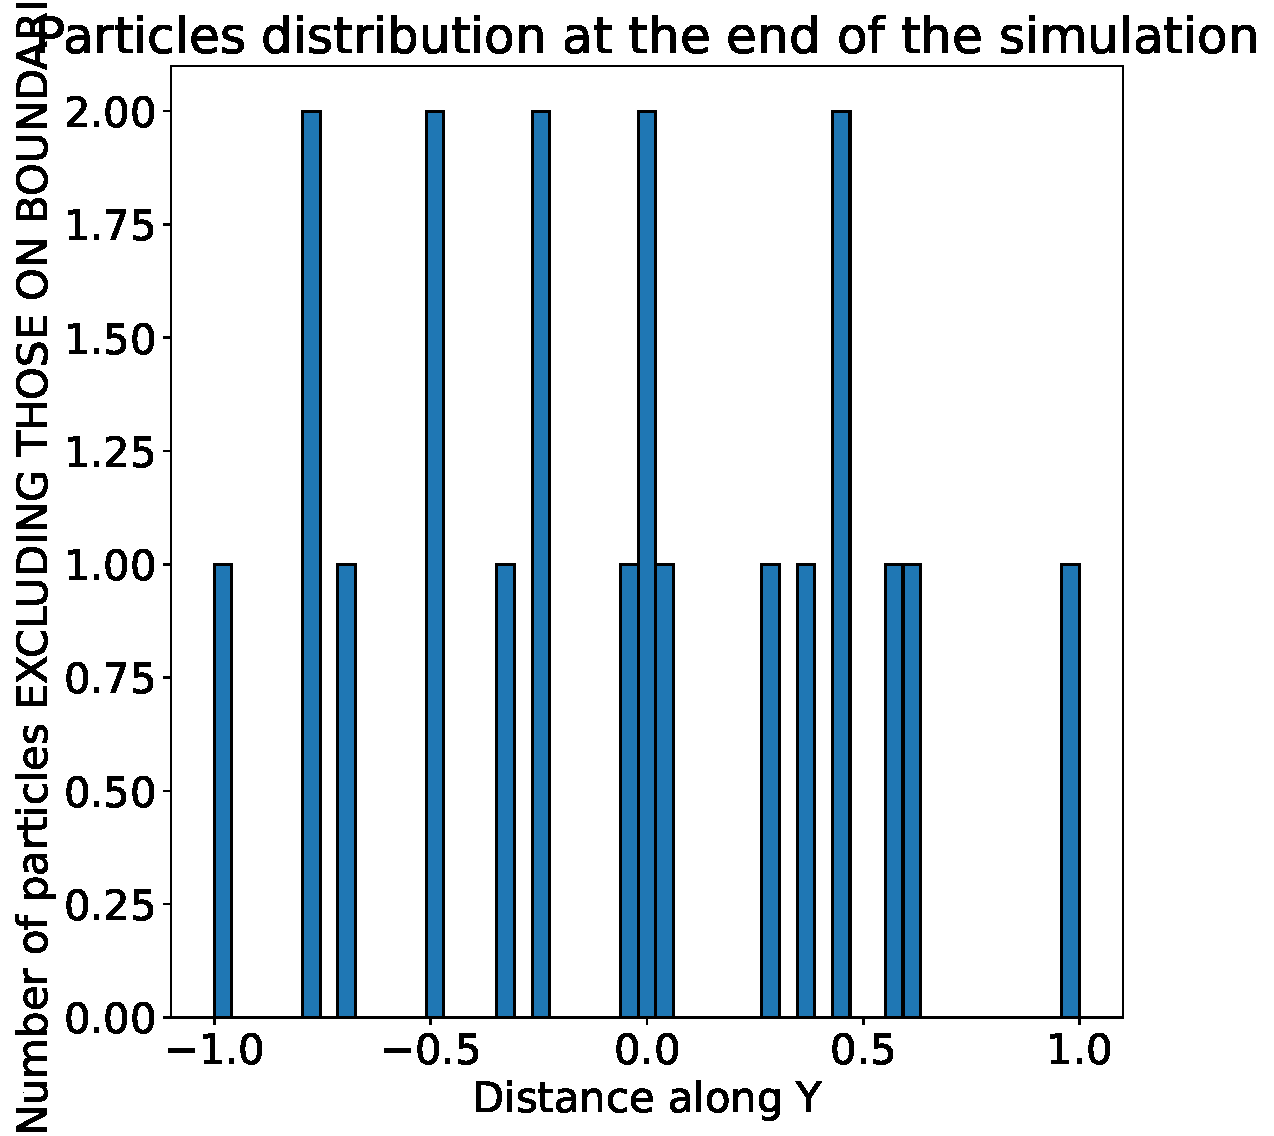
\includegraphics[width=\textwidth]{images/verticalFinalDist.pdf} % Replace with your image path
        \caption{Vertical distribution of particles}
        \label{fig:subplotVertFinal}
    \end{subfigure}
    \hfill
    \begin{subfigure}[b]{0.45\textwidth}
        \centering
        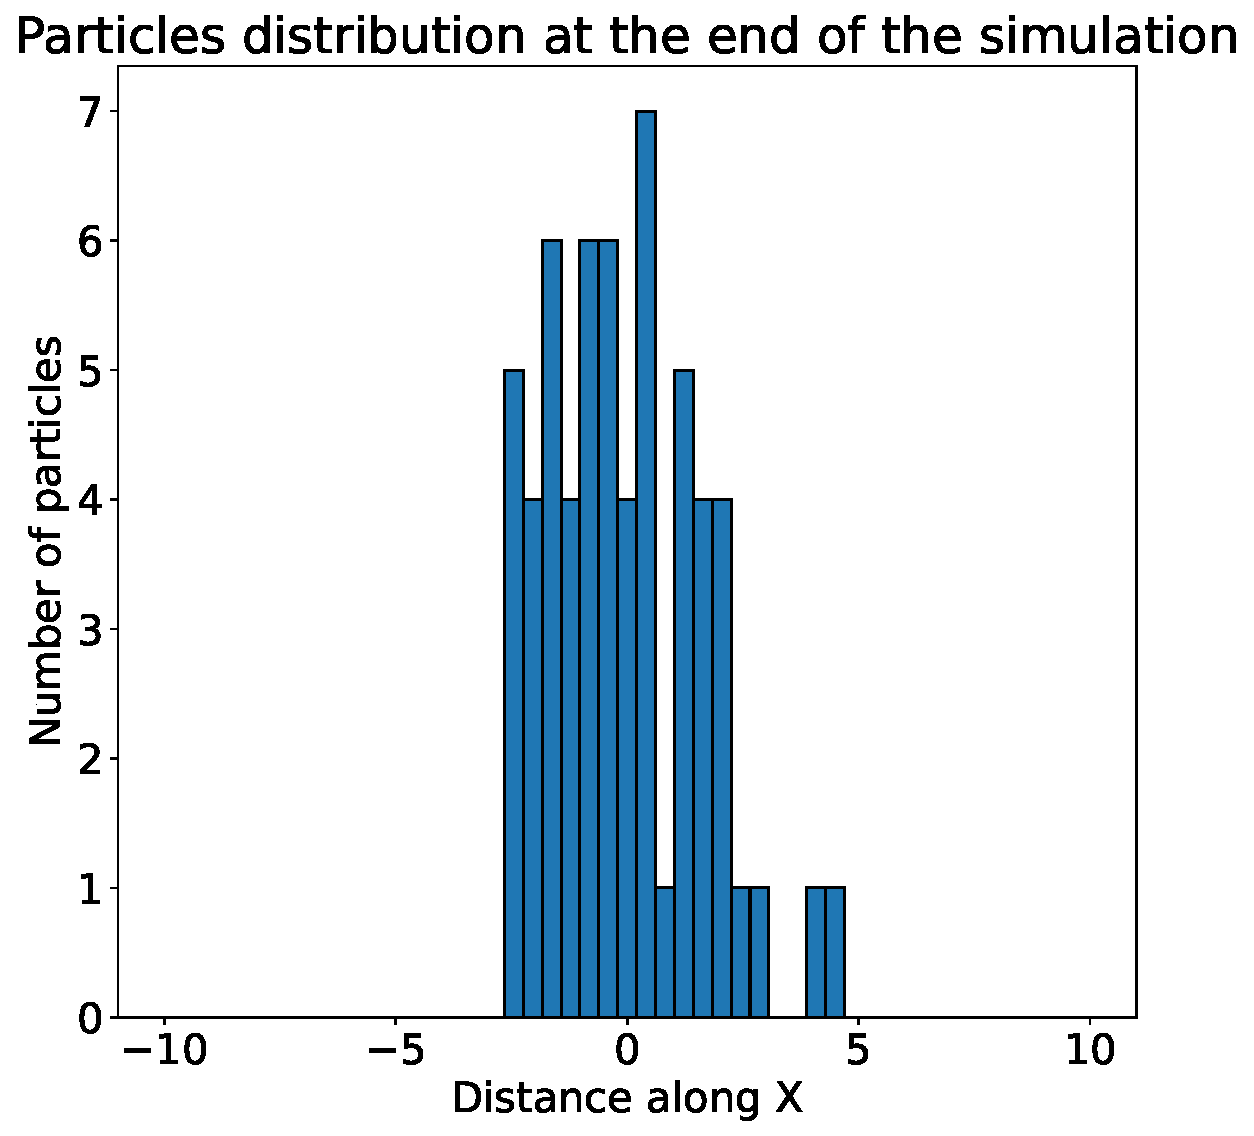
\includegraphics[width=\textwidth]{images/horizontalFinalDist.pdf} % Replace with your image path
        \caption{Horizontal distribution of particles}
        \label{fig:subplotHorFinal}
    \end{subfigure}
    \caption{Absorbing boundaries}
    \label{fig:Absorption}
\end{figure}

\end{document}